\documentclass[10pt]{exam}
\usepackage[phy]{template-for-exam}
\usepackage{tikz,graphicx}

\footer{\small \emph{This lab is based off of Experiment \#7 in PASCO's Introductory Optics System Manual.}}{}{\sc \myclass}


\title{Lens Lab}
\author{Rohrbach}
\date{\today}

\begin{document}
\maketitle

\begin{questions}

  \question Measure the height of the object (the target): \hfill  \fillin[][10em]~mm

  \question You will be using a lens that has a focal length of \textbf{75~mm}.

  \question In a moment, we are going to set up the ray table so that the lens is \textbf{300~mm} away from the object.   \label{firstcalc}

  \begin{parts}
    \part Draw a picture of this situation. \vs

    \part Write down your knowns and unknowns. \vs

    \part Use the Fundamental Lens Equation to calculate what the distance to the image would be. (\emph{This will be the \textbf{expected $\bf d_i$} in the table below.}) \vs

    \part Use the Magnification Equation to determine what the image height will be.  (\emph{This will be the \textbf{expected $\bf h_i$} in the table below.}) \vs


  \end{parts}

\pagebreak

\question Make the same calculations for each of the following situations:
\label{othercalcs}

  \tikzstyle{lensmm}=[]
    \begin{tikzpicture}[x=1.2cm]
      \clip (-1.5,2) rectangle (11.5,3.2);
      \node[lensmm] at (0,3) (i) {\bf Lens is 225~mm};
      \node[lensmm] at (0,2.6) {\bf from object};
      \node[lensmm] at (5,3) {\bf Lens is 100~mm};
      \node[lensmm] at (5,2.6) {\bf from object};
      \node[lensmm] at (10,3) {\bf Lens is 50~mm};
      \node[lensmm] at (10,2.6) {\bf from object};

      \draw (2.5,3.3) -- ++(0,-1);
      \draw (7.5,3.3) -- ++(0,-1);
    \end{tikzpicture}

  \def\tp{

  }

  \begin{parts}
    \part Write down your knowns and unknowns. 
    
    \uplevel{
      \begin{tikzpicture}[x=1.2cm]
        \clip (-1.5,0) rectangle (11,3.2);

        \draw (2.5,3.3) -- ++(0,-4);
        \draw (7.5,3.3) -- ++(0,-4);
      \end{tikzpicture}
    }

    \part Use the Fundamental Lens Equation to calculate what the distance to the image would be. (\emph{This will be the \textbf{expected $\bf d_i$} in the table below.})

    \uplevel{
      \begin{tikzpicture}[x=1.2cm]
        \clip (-1.5,-3) rectangle (11,3.2);

        \draw (2.5,3.3) -- ++(0,-6);
        \draw (7.5,3.3) -- ++(0,-6);
      \end{tikzpicture}
    }

    \part Use the Magnification Equation to determine what the image height will be.  (\emph{This will be the \textbf{expected $\bf h_i$} in the table below.}) 

    \uplevel{
      \begin{tikzpicture}[x=1.2cm]
        \clip (-1.5,-3) rectangle (11,3.2);

        \draw (2.5,3.3) -- ++(0,-6);
        \draw (7.5,3.3) -- ++(0,-6);
      \end{tikzpicture}
    }


  \end{parts}

\pagebreak

\question
Now we need to set up your experiment. Get the following items out of the box:

\begin{parts}
    \part ``Crossed Arrow Target''
    \part ``75mm focal length convex lens''
    \part ``Screen''
    \part Three L-shaped lens holders
    \part The track
    \part The light source
\end{parts}



\question
Transfer all of your calculations from Questions \#\ref{firstcalc} \& \ref{othercalcs} into the appropriate ``expected'' columns in the table below.

\question
Set up the experiment as shown below:

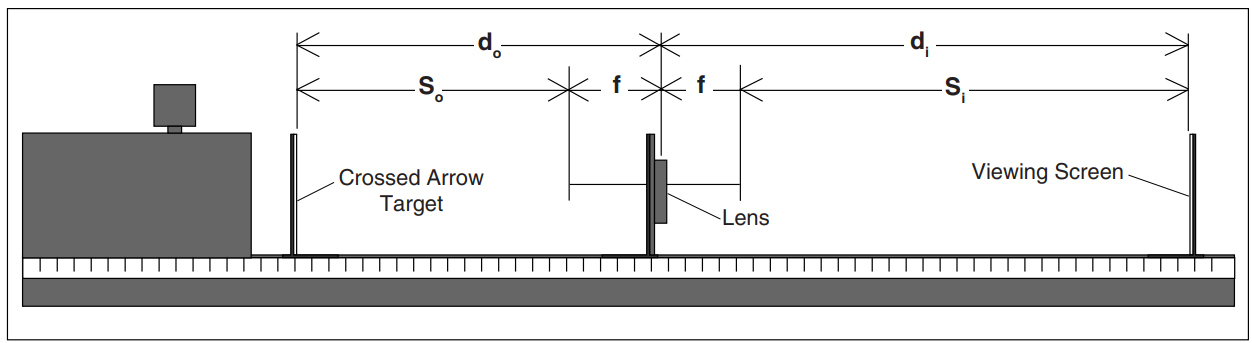
\includegraphics[width=9cm]{Fig7_1.png}

\question
Now, to find the measured values, do the following:

\begin{parts}
    \part To get a $d_o$ of 300 mm (which is equivalent to 30 cm), make the distance between the crossed-arrow target and the lens 30 cm. It does not matter how far the crossed-arrow target is from the light source.
    \part Move the screen until the image comes into sharp focus. Notice that the image is inverted.
    \part Measure the distance between the lens and the screen. This is your \textbf{measured $d_i$}.
    \part Use a ruler to measure the height of the image on the screen. Yes, it will be tiny, but do your best. This is your \textbf{measured $h_i$}. Please note that this value should be \textbf{negative} since the image is inverted.
    \part Repeat the same steps for the other $d_o$ values.
    \part If it is not possible to focus an image on the screen, simply mark an `X' through that box.
\end{parts}


\question
Calculate your percent errors using this equation:
%
\begin{align*}
  \text{\% error} &= 
  \frac{\left| 
    \text{measured} - \text{expected} 
  \right|}{
    \text{expected}
  } 
  \times 100
\end{align*}


\begin{EnvFullwidth}
  \renewcommand{\arraystretch}{3}
  \begin{center}
    \begin{tabular}{|c|c|c|c||c|c|c|}
      \hline
      \textbf{$d_o$ (mm)} & \textbf{$d_i$ expected} & \textbf{$d_i$ measured} & \textbf{\% error} & \textbf{$h_i$ expected} & \textbf{$h_i$ measured} & \textbf{\% error} \\\hline
      300 & & & & & & \\\hline
      225 & & & & & & \\\hline
      100 & & & & & & \\\hline
      50  & & & & & & \\\hline
    \end{tabular}
  \end{center}
\end{EnvFullwidth}

\pagebreak

\question
How good are your percent errors? What are some errors in the experiment that prevent this from being 0\%?

\vs

\question
Which image could not be focused on the screen? Why couldn’t it be focused?

\vs

\question
Looking at your answer to the previous question and the focal length of the lens (75 mm), how is focal length related to whether the image is real or virtual?

\vs

\question
How do your numbers for $d_i$ come out when the image is virtual?

\vs

\end{questions}

\end{document}